\section{Modeling of the DC-Motor}
\todo[inline,author=Jacob]{I'd like to see a block diagram like in next section.}
The purpose of this section is to establish a dynamic model of the DC-motor. This model will result in a transfer function from a voltage input, $U_m$, to an angular velocity output, $\omega_m$. It will be done by modeling the electrical and the mechanical part of the motor and then putting them together to find the transfer function of the motor.

\subsection*{Electrical Model of the Motor}
The electrical circuit of the motor is presented in \autoref{fig:MotorCircuit}.

\begin{figure}[htbp]
	\centering
 	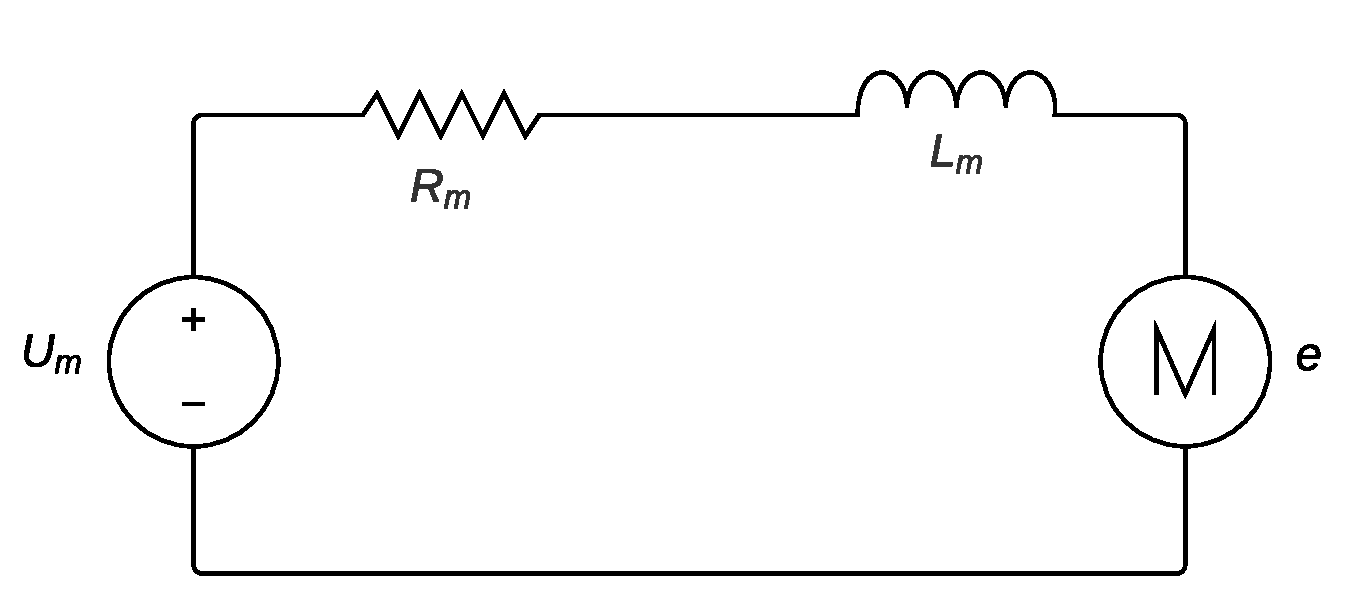
\includegraphics[width=0.7\textwidth]{figures/modeling/Motor/MotorElectricCircuit.pdf} 
 	\caption{Circuit diagram of a DC-motor.}
 	\label{fig:MotorCircuit}
\end{figure}

Using Kirchhoff's voltage law, the electric model of the DC-motor is \autoref{eq:tech_ToA}.
\begin{subequations} \label{eq:tech_ToA}
	\begin{flalign}
		&U_m = R_m \cdot i + L_m \frac{di}{dt} + e \\
		&e = K_e \cdot \omega_m 
	\end{flalign}
\end{subequations}

\startexplain
	\explain{$U_m$ is the voltage output of the generator}{\si{\volt}}
	\explain{$R_m$ is the resistance of the DC-motor}{\si{\ohm}}
	\explain{$L_m$ is the inductance of the DC-motor}{\si{\henry}}
	\explain{$i$ is the current in the DC-motor}{\si{\ampere}}
	\explain{$e$ is the electromotive force}{\si{\volt}}
	\explain{$K_e$ is the motor velocity constant}{\si{\volt\second\per\radian}}
	\explain{$\omega_m$ is the angular velocity of the motor}{\si{\radian\per\second}}
\stopexplain

\subsection*{Mechanical Model of the Motor}
The mechanical free body diagram of the motor is presented in \autoref{fig:MotorBodyDiagram}.

\begin{figure}[htbp]
	\centering
 	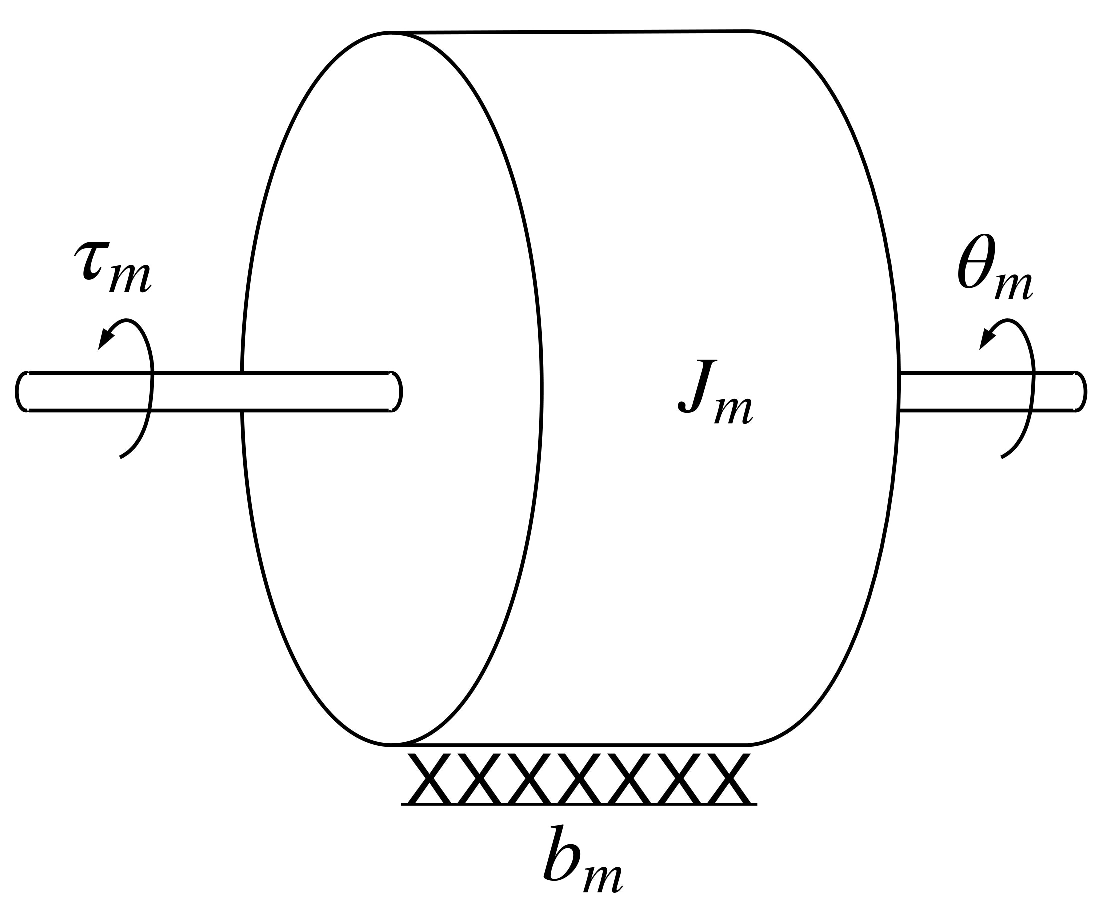
\includegraphics[width=0.4\textwidth]{figures/modeling/Motor/DCMotorMechanic.pdf} 
 	\caption{Free body diagram of a DC-motor.}
 	\label{fig:MotorBodyDiagram}
\end{figure}

When applied to a rotational movement, Newton's second law of motion state that the sum of the torques applied to an object equals the moment of inertia times the angular acceleration of this object. From \autoref{fig:MotorBodyDiagram}, the equation for the mechanical part of the motor is \autoref{eq:MotorMechanical}.

\begin{equation}
	J_{m} \dot{\omega}_{m} = \tau_{m} - \tau_{l} - \tau_{fm}
	\label{eq:MotorMechanical}
\end{equation}

\startexplain
	\explain{$J_m$ is the moment of inertia of the motor}{\si{\kilo\gram\meter\squared}}
	%\explain{$\omega_m$ is the angular velocity of the DC-motor}{\si{\radian\per\second}}
	\explain{$\tau_m$ is the torque of the DC-motor}{\si{\newton\meter}}
	\explain{$\tau_l$ is the torque of the load}{\si{\newton\meter}}
	\explain{$\tau_{fm}$ is the torque of the friction}{\si{\newton\meter}}
\stopexplain

The motor's torque and the friction's torque, respectively $\tau_m$ and $\tau_f$, are defined by \autoref{eq:tauLm}.

\begin{subequations}\label{eq:tauLm}
	\begin{flalign}
		&\tau_m = K_t \cdot i  \label{eq:MotorTorque}\\	
		&\tau_{fm} = b_{m}\cdot\omega_{m}	\label{eq:FrictionTorque}
	\end{flalign}
\end{subequations}

\startexplain
	\explain{$K_t$ is the motor torque constant}{\si{\newton\meter\per\ampere}}
	\explain{$b_m$ is the viscous friction coefficient}{\si{\newton\meter\second\per\radian}}
\stopexplain

Inserting \autoref{eq:tauLm} into \autoref{eq:MotorMechanical} gives \autoref{eq:Jm}.
\begin{equation}
	J_{m} \cdot \dot{\omega}_{m} = K_{t} \cdot i - \tau_{l} - b_{m} \cdot \omega_{m} \label{eq:Jm}
\end{equation}

\subsection*{Combined Model of the Motor}
First the electrical and mechanical equations of the motor are Laplace-transformed in \autoref{eq:MotorLaplace}
\begin{subequations}\label{eq:MotorLaplace}
	\begin{flalign}
		&U_{m}(s) = R_{m} \cdot I(s) + s \cdot L_{m} \cdot I(s) + K_{e} \cdot \Omega_{m}(s) \addunit{1} \label{eq:ElectricalLaplace}\\	
		&s\cdot J_{m} \cdot \Omega_{m}(s) = K_{t} \cdot I(s) - \tau_{l} - B_{m} \cdot \Omega_{m}(s) \addunit{1}	\label{eq:MechanicalLaplace}
	\end{flalign}
\end{subequations}

%The current, I(s), is isolated in \autoref{eq:ElectricalLaplace}:
%\begin{equation}
%	I(s)=\frac{U_m(s)-K_e\cdot\Omega(s)}{R_m+sL_m} \addunit{1}
%	\label{eq:MotorCurrent}
%\end{equation}

%Then \autoref{eq:MotorCurrent} is inserted in \autoref{eq:MechanicalLaplace}:
The current, $I(s)$, is isolated and inserted in \autoref{eq:MechanicalLaplace} giving \autoref{eq:Iinserted}.
\begin{equation}
	s\cdot J_{m} \cdot \Omega_{m}(s) = K_{t} \frac{U_m(s)-K_e\cdot\Omega_{m}(s)}{R_m+sL_m} - \tau_{l} - B_{m} \cdot \Omega_{m}(s) \addunit{1}
	\label{eq:Iinserted}	
\end{equation}

This is the model of the motor but the torque of the load, $\tau_l$, is yet to be determined.